%
%	This is the original file provided by Dominic Corbett on the
%	M337 Forum so that it could be included in the solutions paper.
%
\documentclass[10pt,a4paper]{article}
\usepackage{amsmath}
\usepackage{amsfonts}
\usepackage{amssymb}
\DeclareMathOperator{\re}{Re}
\DeclareMathOperator{\im}{Im}
\usepackage{fullpage}
\delimitershortfall-1sp
\newcommand{\cbr}[1]{\left\{#1\right\}}
\newcommand{\abs}[1]{\left\lvert#1\right\rvert}
\usepackage{lastpage}
\usepackage{tikz}
\usepackage{subcaption}
\usepackage{fancyhdr}
\pagestyle{fancy}
\lhead{M337 --- 2013 Exam Solutions}
\chead{}
\rhead{DBJC}
\headsep = 10pt
\lfoot{}
\cfoot{\thepage\ of \pageref{LastPage}}
\rfoot{}
\renewcommand{\headheight}{12.0pt}
\renewcommand{\headrulewidth}{0.4pt}
\renewcommand{\footrulewidth}{0.4pt}
\definecolor{light-gray}{gray}{0.75}
\definecolor{light-light-gray}{gray}{0.875}
\usepackage{xr-hyper}
\usepackage[bookmarks=true,backref=section,colorlinks=true,linkcolor=black,pdftitle={M337 2013 Exam Solutions},pdfauthor={DBJC}]{hyperref}
\begin{document}
\begin{figure}
	\centering
	\begin{subfigure}{0.49\textwidth}
		\centering
		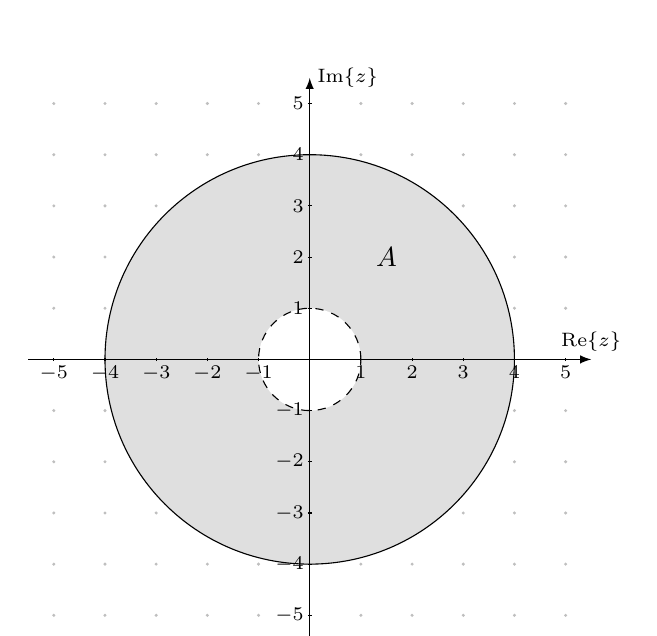
\begin{tikzpicture}[scale=0.65][font=\scriptsize]
			\foreach \x in {-5,-4,-3,-2,-1,1,2,3,4,5}{							% reference grid
				\foreach \y in {-5,-4,-3,-2,-1,1,2,3,4,5}{
					\filldraw [light-gray] (\x,\y) circle (0.5pt) ;
				}
			}
			\draw [draw=black,fill=light-light-gray] (0,0) circle (4);					% outer limit
			\draw [draw=black,dashed,fill=white] (-0,0) circle (1);					% inner limit
			\node[font=\normalsize] at (1.5,2) {$ A $};							% label
			\draw [-latex] (-5.5,0) -- (5.5,0) node [above]  {$\re\{z\}$};				% Real axis
			\draw [-latex] (0,-5.5) -- (0,5.5) node [right] {$\im\{z\}$};				% Imaginary axis
			\foreach \n in {-5,-4,...,-1,1,2,...,4,5}{								% real axis ticks
				\draw (\n,-1pt) -- (\n,1pt)   node [below] {$\n$};
			}
			\foreach \n in {-5,-4,...,-1,1,2,...,4,5}{								% imaginary axis ticks
				\draw (-1pt,\n) -- (1pt,\n)   node [left] {$\n$};
			}
		\end{tikzpicture}
		\caption{Sketch of the set $ A = \cbr{ z : 1 < \abs{ z } \leq 4 } $.}
		\label{setA}
	\end{subfigure}
	\begin{subfigure}{0.49\textwidth}
		\centering
		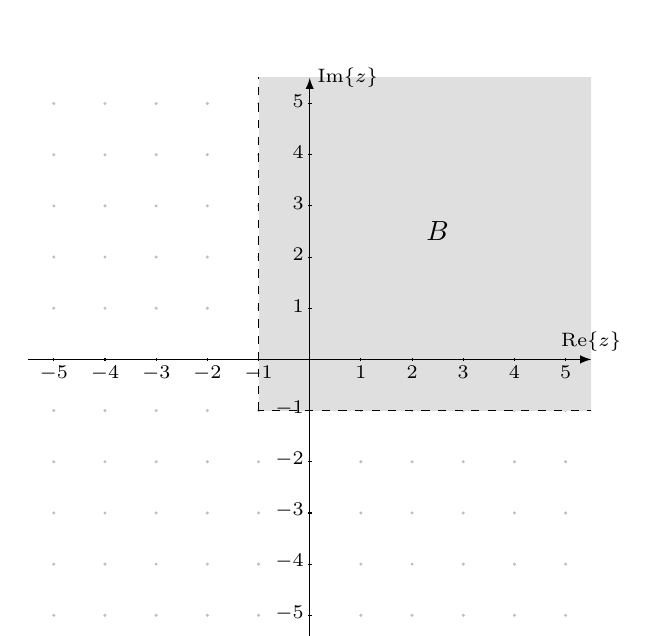
\begin{tikzpicture}[scale=0.65][font=\scriptsize]
			\foreach \x in {-5,-4,-3,-2,-1,1,2,3,4,5}{							% reference grid
				\foreach \y in {-5,-4,-3,-2,-1,1,2,3,4,5}{
					\filldraw [light-gray] (\x,\y) circle (0.5pt) ;
				}
			}
			\begin{scope}
				\clip (-2.5,-2.5) rectangle (5.5,5.5);
				\filldraw [dashed,fill=light-light-gray] (-1,-1) rectangle (6,6);		% excluded boundaries
			\end{scope}
			\node[font=\normalsize] at (2.5,2.5) {$ B $};							% label
			\draw [-latex] (-5.5,0) -- (5.5,0) node [above]  {$\re\{z\}$};				% Real axis
			\draw [-latex] (0,-5.5) -- (0,5.5) node [right] {$\im\{z\}$};				% Imaginary axis
			\foreach \n in {-5,-4,...,-1,1,2,...,4,5}{								% real axis ticks
				\draw (\n,-1pt) -- (\n,1pt)   node [below] {$\n$};
			}
			\foreach \n in {-5,-4,...,-1,1,2,...,4,5}{								% imaginary axis ticks
				\draw (-1pt,\n) -- (1pt,\n)   node [above=0.3mm, left] {$\n$};
			}
		\end{tikzpicture}
		\caption{Sketch of the set $ B = \cbr{ z : \re z > -1 , \im z > -1 } $.}
		\label{setB}
	\end{subfigure}
	\begin{subfigure}{0.49\textwidth}
		\centering
		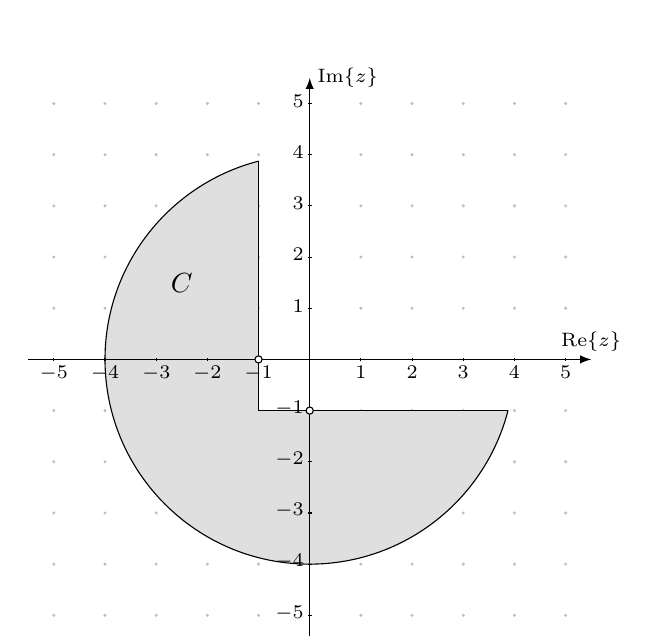
\begin{tikzpicture}[scale=0.65][font=\scriptsize]
			\foreach \x in {-5,-4,-3,-2,-1,1,2,3,4,5}{							% reference grid
				\foreach \y in {-5,-4,-3,-2,-1,1,2,3,4,5}{
					\filldraw [light-gray] (\x,\y) circle (0.5pt) ;
				}
			}
			\begin{scope}
				\clip (-5,-5) -- (-5,5) -- (-1,5) -- (-1,-1) -- (5,-1) -- (5,-5) -- cycle;
				\draw [draw=black,fill=light-light-gray] (0,0) circle (4);				% outer limit
			\end{scope}
			\begin{scope}
				\clip (0,0) circle (4);
				\draw (-1,5) -- (-1,-1) -- (5,-1);								% new boundaries
			\end{scope}
			\node[font=\normalsize] at (-2.5,1.5) {$ C $};						% label
			\draw [-latex] (-5.5,0) -- (5.5,0) node [above]  {$\re\{z\}$};				% Real axis
			\draw [-latex] (0,-5.5) -- (0,5.5) node [right] {$\im\{z\}$};				% Imaginary axis
			\foreach \n in {-5,-4,...,-1,1,2,...,4,5}{								% real axis ticks
				\draw (\n,-1pt) -- (\n,1pt)   node [below] {$\n$};
			}
			\foreach \n in {-5,-4,...,-1,1,2,...,4,5}{								% imaginary axis ticks
				\draw (-1pt,\n) -- (1pt,\n)   node [above=0.3mm, left] {$\n$};
			}
			\filldraw [fill=white] (-1,0) circle (2pt);								% excluded points
			\filldraw [fill=white] (0,-1) circle (2pt);
		\end{tikzpicture}
		\caption{Sketch of the set $ C = A - B $.}
		\label{setC}
	\end{subfigure}
	\begin{subfigure}{0.49\textwidth}
		\centering
		\begin{tikzpicture}[scale=0.65][font=\scriptsize]
			\foreach \x in {-5,-4,-3,-2,-1,1,2,3,4,5}{							% reference grid
				\foreach \y in {-5,-4,-3,-2,-1,1,2,3,4,5}{
					\filldraw [light-gray] (\x,\y) circle (0.5pt) ;
				}
			}
			\draw (-1,5.5) -- (-1,-1) -- (5.5,-1);								% boundary
			\node[font=\normalsize] at (-1.5,1.75) {$ D $};						% label
			\draw [-latex] (-5.5,0) -- (5.5,0) node [above]  {$\re\{z\}$};				% Real axis
			\draw [-latex] (0,-5.5) -- (0,5.5) node [right] {$\im\{z\}$};				% Imaginary axis
			\foreach \n in {-5,-4,...,-1,1,2,...,4,5}{								% real axis ticks
				\draw (\n,-1pt) -- (\n,1pt)   node [below] {$\n$};
			}
			\foreach \n in {-5,-4,...,-1,1,2,...,4,5}{								% imaginary axis ticks
				\draw (-1pt,\n) -- (1pt,\n)   node [above=0.3mm, left] {$\n$};
			}
		\end{tikzpicture}
		\caption{Sketch of the set $ D = \partial D $.}
		\label{setD}
	\end{subfigure}
	\caption{Sketches of the sets $ A $, $ B $, $ C $, and $ D $.}
	\label{2aSketches}
\end{figure}
\end{document}
